\documentclass[a4paper,12pt]{article}
\usepackage{fancyhdr}
\usepackage{lastpage}
\usepackage{geometry}
\usepackage{listings}
\usepackage{datetime}
\usepackage{xeCJK}
\usepackage{hyperref}
\usepackage{amsmath}
\usepackage{graphicx}
\usepackage{float} % 加入 float 宏包以使用 [H]
\usepackage{longtable}

\geometry{left=2.5cm, right=2.5cm, top=2.5cm, bottom=2.5cm}
\pagestyle{fancy}
\setCJKmainfont{Noto Sans TC}
% 英文字體 consolas
\setmonofont{Consolas}
% 設定內文文字大小
\renewcommand{\normalsize}{\fontsize{12pt}{\baselineskip}\selectfont}

% 設定頁首
\fancyhf{}
\fancyhead[L]{Volume Rendering and Gradient Visualization(HW2)}
\fancyhead[R]{\today}
\fancyfoot[C]{\thepage/\pageref{LastPage}}

\title{Volume Rendering and Gradient Visualization(HW2)}
\author{01057033洪銘均}
\date{\today}

\begin{document}
\maketitle
\tableofcontents
\newpage

\section{程式概述}
該程式使用Sammon Mapping將信用卡交易資料特徵進行降維,並利用紅色、藍色標註可疑交易及普通交易,以方便觀察兩種交易降維後的關係


\section{運行結果}

\begin{figure}[H]
    \centering
    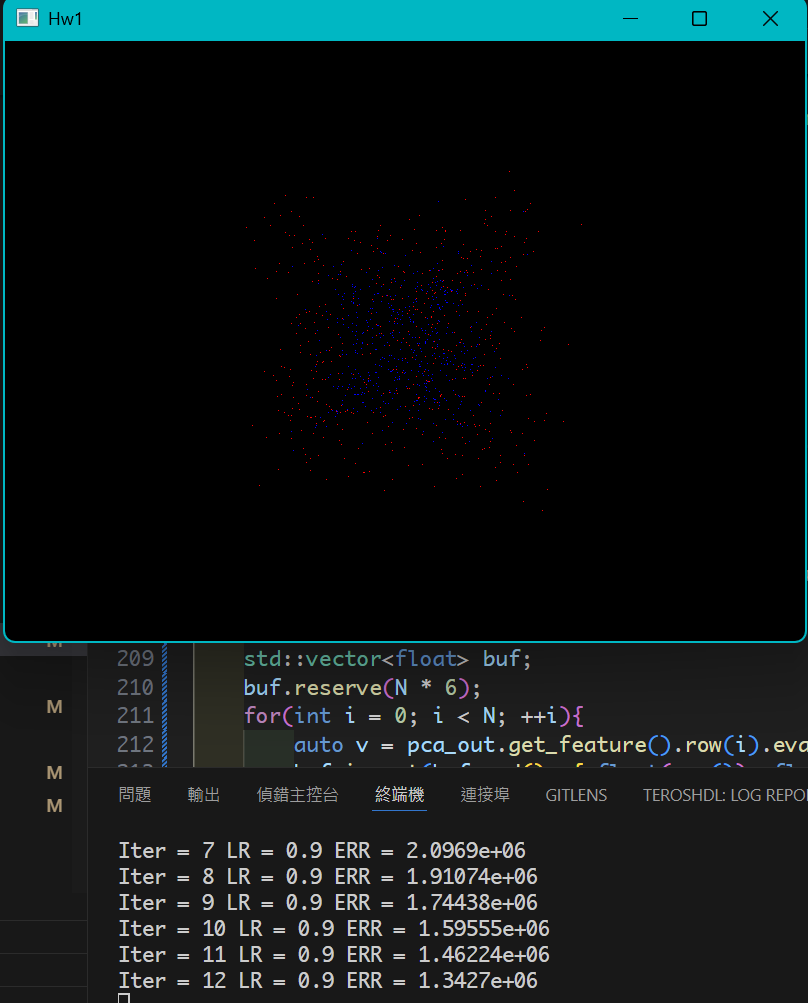
\includegraphics[width=0.8\textwidth]{img/img2.png}
\end{figure}\\
Sammon Mapping開始時可以看到紅色與藍色點的位置相對隨機,藍色與紅色並未顯示出分群等特徵


\begin{figure}[H]
    \centering
    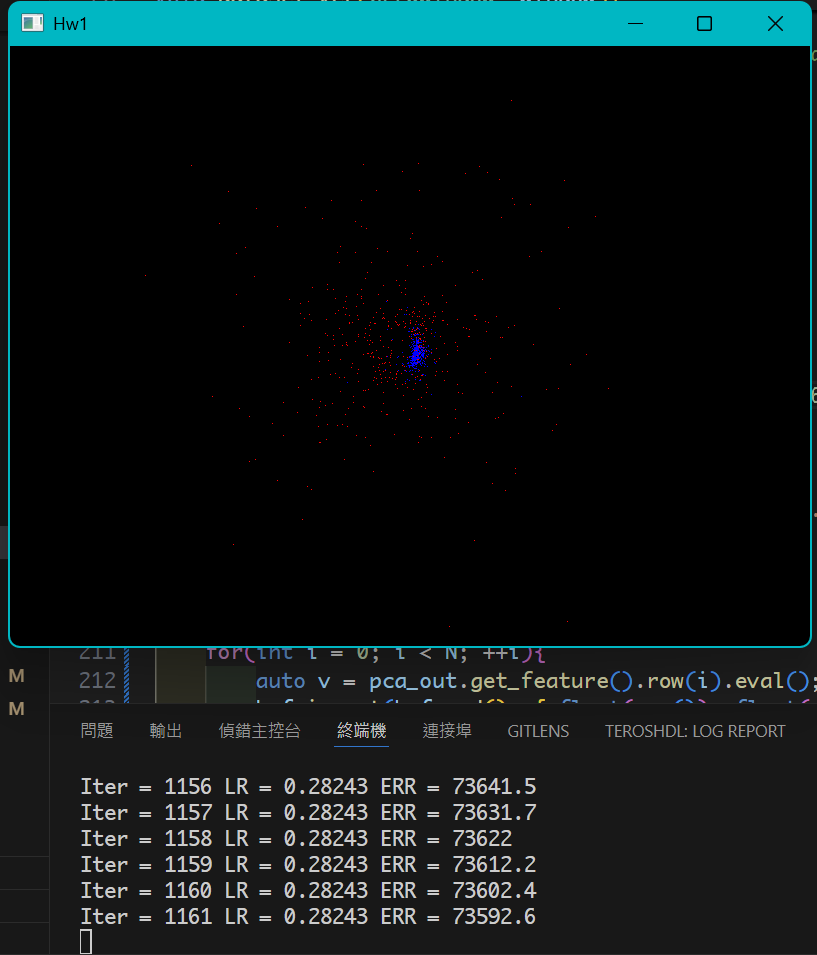
\includegraphics[width=0.8\textwidth]{img/img0.png}
\end{figure}\\
經過1000多次的Iteration可以看到藍色與紅色出現明顯的差異特徵,藍色集中在畫面中間,但紅色則大量散佈在畫面各處,可以看出來Sammon mapping確實有對資料之間的關係進行分群,在降維後依舊保留特徵

\begin{figure}[H]
    \centering
    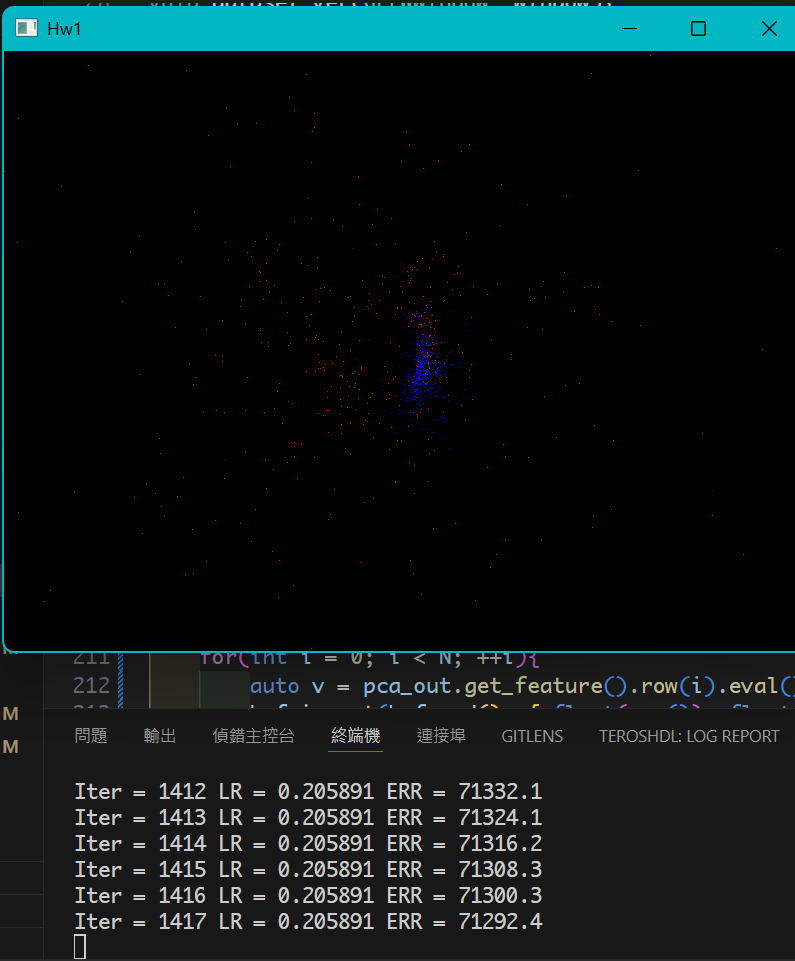
\includegraphics[width=0.8\textwidth]{img/img1.png}
\end{figure}\\
局部放大後可以看到藍色相對集中



\section{心得}
    這次作業將高維度資料進行降維,在Iterate過程中可以看到資料快速分群,後續資料也只是稍微震盪,在一開始知道這方法時我以為只能使用深度學習等方法才能判別這類高維度資料的資料特徵,但這次作業利用Mapping等方式也讓我理解到傳統的方法是如何做資料識別的,在未來若有相關深度學習可能可以參考降維等方法做預處理。
\end{document}

% xelatex  --max-print-line=10000 -synctex=1 -interaction=nonstopmode -file-line-error -recorder .\codebook.tex 
